\section{PRACTICAL IMPLEMENTATION}

This section presents the practical implementation of the gamified educational site designed to introduce learners to the Open Badges of the already completed project. 
The implementation phase is meant to transfer the previously established concepts and structure into an interactive, web-based application. 
The implementation section is concerned with reviewing the design process, approach and technical and design requirements, as well as the integration of gamification elements within the individual sections of the website. 
Certain components of frontend and backend code and the visual elements of the website will be reviewed further in-depth. 
Finally, technical limitations encountered during the development of the implementation will also be discussed. 
The following are the outline of the main design steps taken throughout the project.

\subsection{Layout Decisions}
In the early design phase of the gamified educational website low-fidelity wireframe designs were created to explore potential layout logic, user interaction flow and screen constraints, specifically for a mobile-first layout. 
These initial prototypes were developed using primarily digital mockups via the tool Figma, such as the one shown in \ref {fig:mockups}, which represents a series of mobile screen layouts for each gamified task stage. 
Wireframes played a crucial role in identifying key user interface (UI) elements, narrative progression, and functional zones for gamified interaction.

\begin{figure}[H]
  \centering
  \begin{subfigure}[]{0.3\textwidth}
    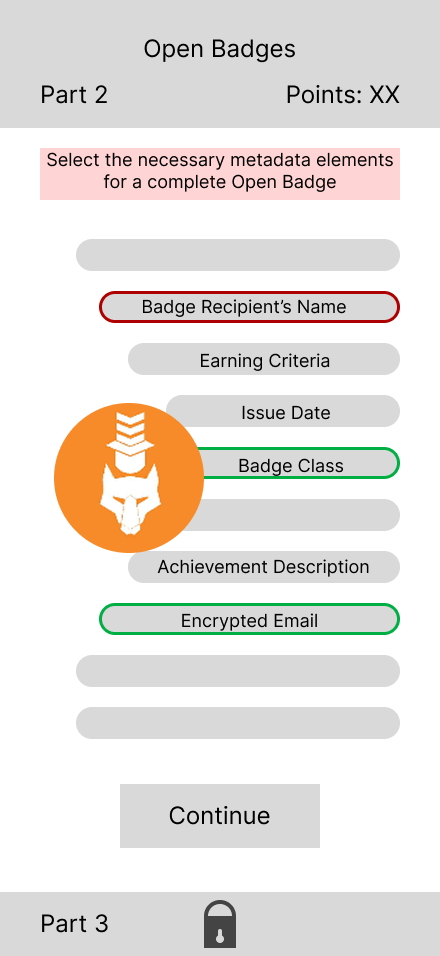
\includegraphics[width=\textwidth]{Media/design1.png}
    \caption{Task 1: Metadata selection}
  \end{subfigure}
  \hfill
  \begin{subfigure}[]{0.3\textwidth}
    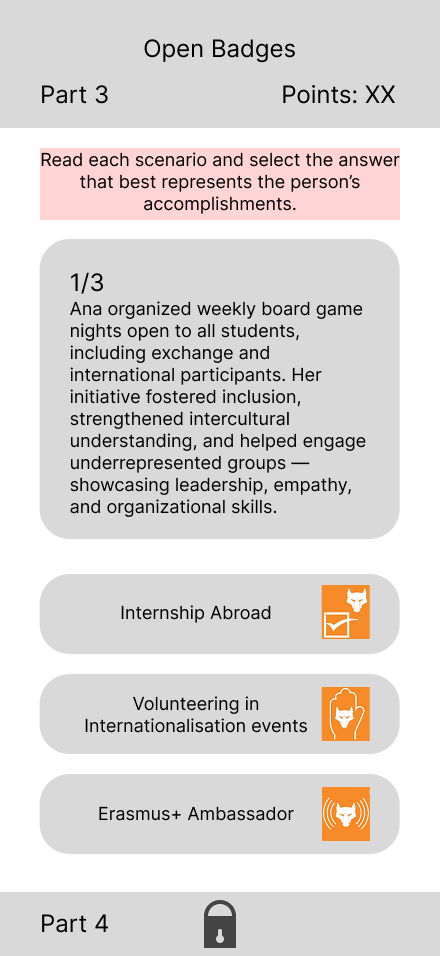
\includegraphics[width=\textwidth]{Media/design2.png}
    \caption{Task 2: Scenario choice}
  \end{subfigure}
  \hfill
  \begin{subfigure}[]{0.3\textwidth}
    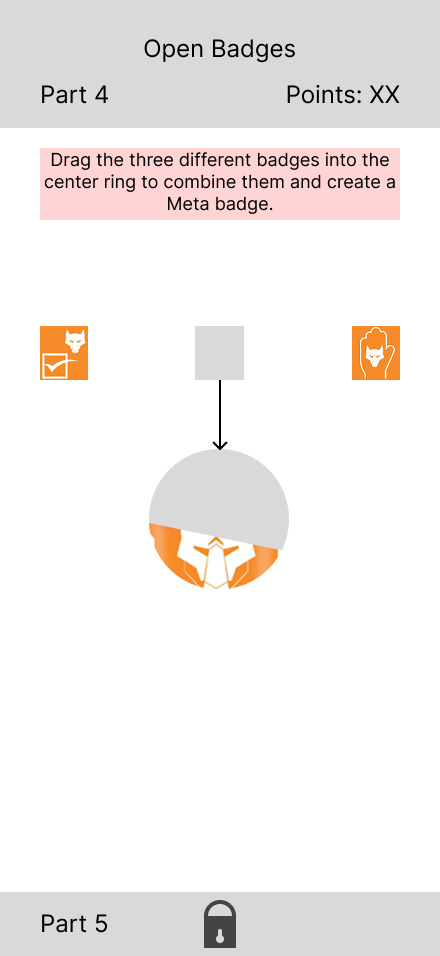
\includegraphics[width=\textwidth]{Media/design3.png}
    \caption{Task 3: Meta badge creation}
  \end{subfigure}
  \caption{Mobile UI mockups showing key gamified tasks}
  \label{fig:mockups}
  {\raggedright \small{Source:} created by the author\par}
\end{figure}

Early in the design stage, the usage of Phaser 3 for a game experience within the website was left behind, due to the concerns that it could stigmatise Open Badges by associating them with video games. 
After an in-depth discussion with the supervisor, to avoid this stigma, Phaser 3 segments have been entirely cut from the project.

The overall layout of the gamified website was designed to support focused, step-by-step learning with minimal distraction. 
Some of the decisions were due to technical reasons; others, like a one-page structure, were product requirements specified by the supervisor.
Each design decision is made with the goal to emphasise clarity, responsiveness, and gamified interactivity, aligning both with pedagogical goals and user experience standards.

\subsubsection{Detailed Design Decisions}

\begin{itemize}
    \item \textbf{One-Page Scrollable Structure}: The website is a single scrollable page to maintain narrative continuity and reduce navigation complexity. 
    This promotes immersion by guiding users through a structured sequence without requiring manual or automatic page changes and allows for a strictly guided experience. 
    It also allows for lazy loading\footnote{A form of pre-loading where the website is instructed to load resources only when extra throughput is available and the core elements that the user is viewing are already loaded.} of visual elements such as the merge animation video that improves the stability and performance of the website.
    \item \textbf{Scroll Snapping Between Sections}: Scroll snapping was explored in-depth, and originally it was intended to lock the full website in scroll-snapping, but further investigation lead to poor performance for either mobile or desktop users. 
    While the website is intended as mobile-first, creating a poor experience for the rest of the users is not viable or reasonable here, and so instead a series of anchor systems and respective elements were designed alongside a set of buttons to scroll between them. 
    In essence, each section holds an anchor <div> vertical element of the size of 1 pixel with respective offsets. 
    Each task has a button that either aligns the task to fill up the screen fully and consistently for the user or aligns the content for more comfortable reading. 
    It works in each task individually, but there are additional buttons that help traverse sections at the start and end of the website. 
    This technique reinforces the concept of discrete “levels” or learning stages and prevents partial, out-of-context views of adjacent sections.
    \item \textbf{Task-Based Segmentation}: Content is divided into modular, self-contained tasks, each with its own interactive mechanics and feedback. 
    This segmentation mirrors gamification principles, providing a clear sense of progress and achievement at each step. 
    It functions as a level-based system that the user gets to progress through.
    \item \textbf{Mobile-First Responsive Layout}: The interface was designed from the beginning to function on small screens, due to around 70\% of websites today being viewed on a mobile device according to Research.com \footnote{https://research.com/software/guides/mobile-vs-desktop-usage}. 
    Interactive elements are touch-optimised, which is discussed later in more detail. 
    Additionally, elements are vertically stacked, and dynamically scaled, ensuring usability across a range of devices.
    \item \textbf{Colour-Guided Interactivity}:  The interface uses distinct colour signals (deep blue, yellow, green/red) to distinguish structural elements, guide attention, and provide immediate correctness feedback, supporting an intuitive, quick, comprehensible, and accessible user experience.
    \item \textbf{Integrated Feedback and Visual Cues}:  Feedback mechanisms such as visual popups, overlays, task completion percentages, score increases or decreases, animation effects and visual flair such as the vertical zigzag following user-scrolling during the introduction section are embedded into the layout in ways to empower the user and respectively guide them through the experience. 
    These reinforce user actions and promote continued engagement.
    \item \textbf{Content Locking and Sequential Unlocking}:  Later sections remain inaccessible until previous tasks are completed, reinforcing a mastery-based progression model. 
    This prevents skimming or skipping ahead and encourages focused engagement with each concept.
\end{itemize}

\subsection{Element Design}
The design of individual interface elements throughout the website was primarily function-driven, where aesthetic decisions were made to support clarity, usability, and user feedback. 
Colours, shapes, and placements were selected not for ornamentation but to reinforce interaction goals, task structure, and user guidance. 
Typography was deliberately left minimal, relying on system defaults for simplicity and consistency across devices.

The visual identity of the website was structured to align with the university's branding while enhancing usability through consistent colour coding. 
Deep blue serves as the primary institutional theme colour, providing structural consistency across navigation, section headers, and tasks. 
Yellow is used as an accent to direct attention, applied to call-to-action, or \acrshort{cta} buttons and instructional highlights such as task descriptions, or form submission and website reset buttons. 
As an established interface design principle, green and red are used to indicate task correctness for immediate, intuitive feedback to learners. 
This structured use of colour reduces cognitive load and reinforces motivation by making task outcomes clear.

Elements were laid out in a vertically stacked structure, optimised for mobile interaction, with touch-friendly zones, consistent padding to ensure accessibility across devices. 
These spatial choices were supported by scroll-activated features, such as an animated Scalable Vector Graphics, or \acrshort{svg} zigzag path and progressive unlocking of tasks, that visually signal user advancement. 
Conversely, a website reset is available after completion, which triggers a complete fadeout upon resetting user progress, to better convey the outcome. 
These mechanisms were designed not merely for aesthetics but to support learner motivation and focus, aligning with gamification principles that emphasise immediate, goal-oriented feedback as defined by \cite{redefinition}.

Buttons were styled using a visual hierarchy based on their function. 
Primary actions, such as progressing through tasks or claiming a badge, are styled as yellow, circular buttons, ensuring high contrast and immediate visibility. 
These stand in contrast to outlined or subdued secondary buttons in deep blue, which are used for auxiliary navigation within tasks or task buttons themselves. 
This hierarchy reduces the likelihood of user confusion and subtly guides attention toward key learning actions.

Interactive zones within tasks were also shaped by their function. 
For example, drag-and-drop areas are outlined with dashed or shaded containers to suggest manipulability, while static information zones are clean and visually neutral. 
Pop-up feedback components, such as correction prompts or success confirmations, follow a consistent form with a lightly elevated overlay with clear textual content and contextual visual cues. 
These design elements help distinguish between active, passive, and reactive interface components, enhancing overall clarity.

Finally, the visual hierarchy of the system is intentionally kept thin. 
Task screens aim to present no more than two or three levels of importance at any time (e.g., a task prompt and an interaction area, optional tooltip). 
This supports cognitive load minimisation and aligns with pedagogical priorities, critical in gamified learning contexts where distraction can reduce instructional effectiveness (\cite{reduceDistraction}).

\subsection{Frontend Architecture and Technologies}

The core frontend technologies used for the gamified educational website are HTML, CSS, JavaScript and the JavaScript framework React.js. 
This allowed for a convenient component-based architecture where each task, section or complex element can function as a self-contained, interactive module. 
This can be seen in Figure \ref{fig:app_composition}. 
There, the full structure of the website is visible in code format.
Below is an overview of the implemented tasks, other solutions and the technical and pedagogical strategies employed in their design.

\begin{figure}[htbp]
 \centering
 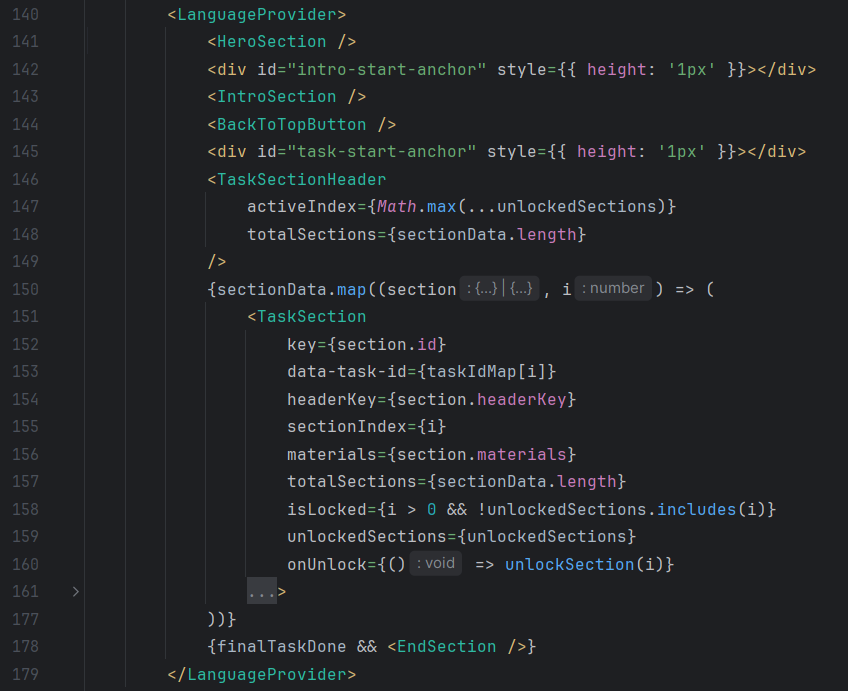
\includegraphics[width=14cm]{Media/app_composition.png}
 \caption{High-level architecture of the website's code components}
 \label{fig:app_composition}
 {\raggedright \small{Source: created by the author, file src/App.js, 2025}\par}
\end{figure}

\subsubsection{Introductory Section}
The hero landing area is designed to give the visitor a very quick impression of the website being related to their recognition through Open Badges, with some visual flair, therefore, it has a bright, deep blue background. 
Some of the basic elements other than headers are a localisation switch between English and Lithuanian, as well as an "About Us" section. 
Due to it being relatively lightweight, it has been developed as a slide-out to reduce clutter as well as maintain the one-page technical requirement. 
Notably the intention within the hero area is to get the user to begin with their progression as quickly as possible. 
A timer is running upon landing within the website that displays a "staircase" of keywords such as "Metadata", "Proof", "Value" and "Skill". 
This guides the user's attention down the page, where a pulse animation plays on the "Start" button, ideally causing the user to begin their journey. 
Upon clicking, the user is scrolled to a display of the introductory section, which is concerned with telling the user only the very core facts about the website:

\begin{itemize}
    \item What is the goal of this website?
    \item How to succeed?
    \item Explanation of how points work.
    \item Core progress tracking information.
\end{itemize}

To better maintain the user's attention, a scroll-linked \acrshort{svg} path follows the user along the existing <div> blocks, signifying the user's progress through the introduction. 
The section is capped off with another \acrshort{cta} button to align the user for the first task.

\subsubsection{Task Section}

To simplify development and maintain consistency and clean code principles and separation of concerns across tasks, each individual task component only implements the interaction logic and content-specific functionality. 
The remaining UI and elements are deferred to the parent TaskSection component. 
As demonstrated in Figure \ref{fig:task_layout}, a typical task component only renders localised instructional prompts, the interactive task UI (e.g., swiper, drag/drop area) as well as a conditional "Continue" button and score bubble. 
The task component is passed props like onUnlock from TaskSection, which allows it to notify the parent when the task has been completed.
The task component also has access to translated strings, session score handling, and internal states such as completed, locked, and selected answers, but these are contained within the component's internal logic.
This architecture makes it easy to expand the system. 
Any new task needs only to adhere to its own specific task content, call onUnlock() when done, and include localised prompts or completion messages. 
Each task is individually fed with a custom order and amount of text headlines and paragraphs to function as the "Materials" of the task, that is then dynamically formatted based on each task.
As a result, each task remains pedagogically distinct yet structurally consistent, ensuring a unified learning experience while supporting varied forms of gamified interaction.

\begin{figure}[hbtp]
\centering
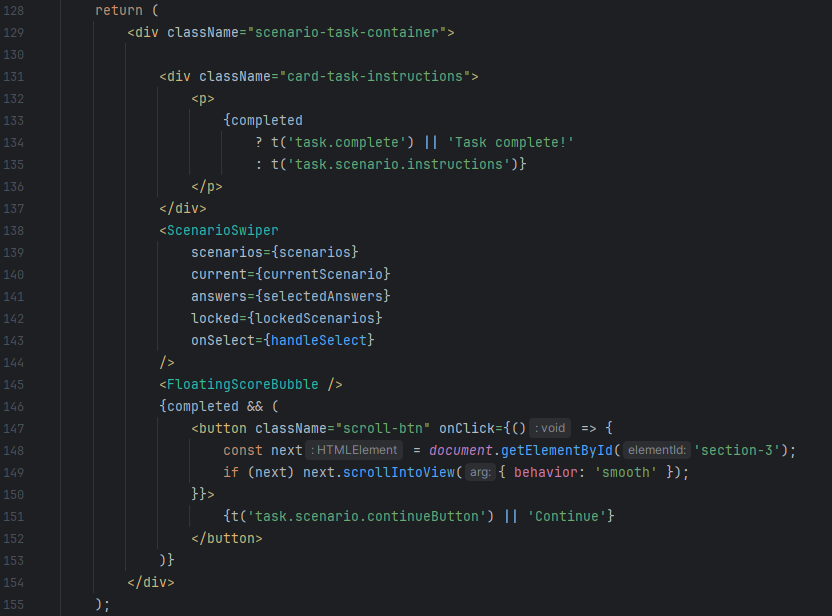
\includegraphics[width=0.8\textwidth]{Media/task_layout.png}
\caption{Code structure of the Scenario task component.}
\label{fig:task_layout}
{\raggedright \small{Source: created by the author, file src/tasks/slidingTask.js, 2025}\par}
\end{figure}

The website implements a browser-based, lightweight system for progress tracking, scoring, and user behaviour logging. 
This approach allows for responsive interactivity while avoiding the need for server-side user accounts, keeping the experience more private and fast.

\textbf{Other modular functionality on the website}:
\begin{itemize}
    \item \textbf{Local storage and progress tracking}: The website tracks user preferences and progress within the local storage of the browser that persists throughout reloads. 
    The preferences specifically track the language selected at the start and if adjusted, will always load the respective language saved.
    Each task section completion is tracked individually through local state as well.
    When a task is completed, a save function is called which adds a statement to the local storage in \acrshort{json} format with a respective identifier, e.g. taskCompletion: \{"task.card-sort":true\}. 
    Should the user reload the website, the task will autocomplete, without tampering with the user's original score.
    This information is then referenced using isTaskCompleted() function to conditionally unlock future sections in the learning path, maintaining the progression model. 
    As mentioned the user's score is also consistently tracked and updated within local storage upon completion of any section.
    Tracking the score only upon completion allows for avoiding score recalculation if the user restarts any section by reloading. 
    This storage solution is ideal for a consistent, clean and private experience, as no actual user PII \footnote{Personally Identifiable Information} is retained.
    \item \textbf{Score system}: The score system operates entirely on the frontend, with a central live score variable that syncs to both persistent storage and UI elements at specific moments. 
    The user’s current score is displayed dynamically and updated in real-time using a custom hook, useLiveScore(), which polls the live score value at the top of the screen throughout the task section. 
    Visual feedback for user actions, such as gaining or losing points upon selecting a correct or incorrect answer respectively is provided via useFloatingScore(). 
    That function triggers a dynamic function element which briefly displays the score delta using a styled floating element near the top of the screen, just below the total live score. 
    The element is either in deep blue to associate with correctness and progress, or red to indicate a mistake.
    The positioning allows the user to associate the score delta with the total score. 
    This feedback is implemented to enhance engagement and give learners further immediate confirmation of their choices.
    The score adjustments are called via adjustScore() function, which then triggers any and all necessary events as seen in Figure \ref{fig:score_update}.
    The user's total score is saved locally upon each task completion and after claiming the Open Badge is attached to the badge issuing request as a criteria addendum, to be discussed later.
    
\begin{figure}[hbtp]
\centering
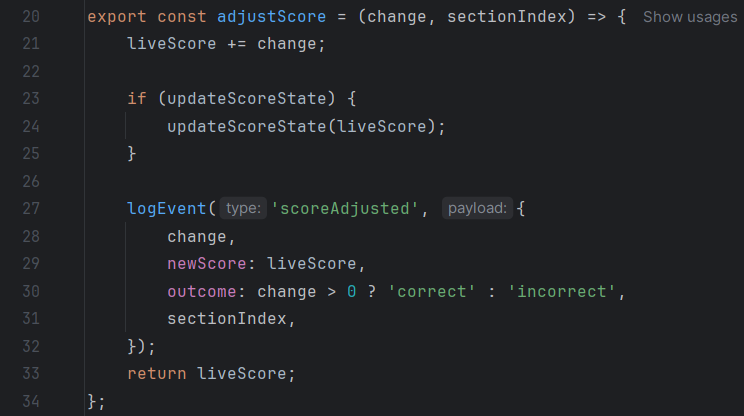
\includegraphics[width=0.8\textwidth]{Media/score_update.png}
\caption{adjustScore() function used to update user score and log outcomes}
\label{fig:score_update}
{\raggedright \small{Source: created by the author, file src/utils/scoreUtils.js, 2025}\par}
\end{figure}

    \item \textbf{Logging of the user's experience}: The system logs significant user interactions via a dedicated event logger module. 
    Each task unlock, score adjustment, or badge claim is recorded with a timestamp and optional payload metadata, as seen in Figure \ref{fig:logging}. 
    The log is stored in memory as a simple JavaScript array, allowing it to be serialised and submitted to the backend for future analysis. 
    This logging framework provides value for both quantitative evaluation of learning engagement later on and debugging during development. 
    These logs are collected and submitted upon submission of the badge claim form, delivering it in \acrshort{json} format to the backend.
\begin{figure}[hbtp]
\centering
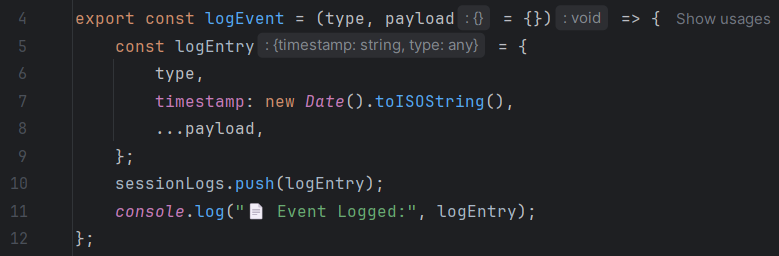
\includegraphics[width=0.8\textwidth]{Media/logging.png}
\caption{logEvent() function, which is responsible for appropriate formatting and creation of each significant interaction log, utils/eventLogger.js, 2025}
\label{fig:logging}
\end{figure}
    \item \textbf{Task question randomisation}: The following feature has been implemented based on feedback during mid-development from supervisors. 
    To improve task replayability and reduce answer memorisation, all tasks implement a randomisation strategy. 
    As seen in Figure \ref{fig:shuffling}, each array of questions and/or their answers is reshuffled within each load, using the shuffleArray() utility function. 
    This ensures that the item order is unpredictable between sessions. 
    For example, the scenario task will present the scenarios in random order, with the answers randomly rearranged, or the metadata task will display a randomly rearranged list of the metadata elements.
\end{itemize}

\begin{figure}[hbtp]
\centering
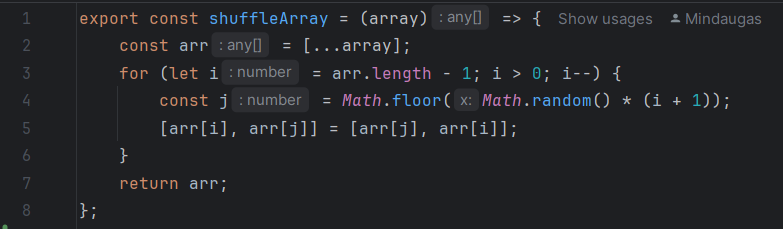
\includegraphics[width=0.8\textwidth]{Media/shuffling.png}
\caption{shuffleArray() function for randomizing answer and question order}
\label{fig:shuffling}
{\raggedright \small{Source: created by the author, file src/utils/shuffle.js, 2025}\par}
\end{figure}

The sequence of tasks was deliberately structured to progressively introduce key concepts surrounding Open Badges through interactive learning. 
Task 1 introduces the idea that badges are closely tied to specific skill recognition, particularly soft skills often overlooked in formal credentials. 
The task challenges the user to differentiate which skills the Open Badges represent. 
Task 2 is more formal and is focused on the required metadata embedded in each badge, which guarantees transparency and verifiability. 
Task 3 shifts to contextual evaluation, where users explore real-world scenarios and relevant badge issuance and reflect on the multiple competencies a single badge might represent. 
Task 4 introduces the idea of badge curation by demonstrating how individual badges can be merged into "Meta" or "Uber" badges that reflect broader or combined achievements. 
Finally, Task 5 shows Open Badges from the perspective of both students and employers, emphasising their dual value as a tool for personal development and recognition. 
This user journey of tasks builds a narrative that is meant to introduce and explain all of the core elements surrounding Open Badges.


\textbf{Task 1: Card Sorting}

The first interactive activity on the website is a card sorting task designed as a basic classification task. 
In this task, users are presented with a bank of draggable skill statements from the "Skills" field.
They must be sorted into one of two columns, labelled as "hard" and "soft" skills. 
Correct placements result in green visual confirmation, score increase and the card becoming fixed in place, while incorrect placements trigger red highlights, a deduction in points with a score deduction bubble, and a contextual explanation overlay. 
Incorrect cards remain draggable, allowing the user to correct their mistake, supporting mastery through trial and error.

The task utilizes the @dnd-kit/core library.
It's a lightweight and extensible drag-and-drop toolkit for React. 
This library was chosen for its strong support of mobile and touch devices, which is critical for a mobile-first layout. 
The main component wraps its content in a <DndContext> element, which handles drag state and event resolution across all draggable and droppable zones. 
Each card is wrapped individually in a DraggableCard component utilising useDraggable(). 
This function allows dragging of the element on both mobile and desktop devices without creating a jarring experience, such as accidentally scrolling with the card. 
Each column is then rendered through DroppableColumn, powered by useDroppable().
A drag event is resolved within the handleDragEnd() function, which determines whether the dragged card was placed into the correct column based on its intended column. 
Correct placements trigger the adjustScore() function with a positive value, and incorrect attempts deduct points and trigger the feedback modal, displaying an instructional message linked to the card’s mistakeKey. 
The card bank is randomised using the shuffleArray() utility on load, reducing memorisation of answer locations between attempts.
The task prompt styled in yellow is located between the columns and skills bank, vertically, to clearly instruct the user and draw necessary attention.
The in-progress task view can be seen in Figure \ref{fig:cardTask}.

\begin{figure}[hbtp]
\centering
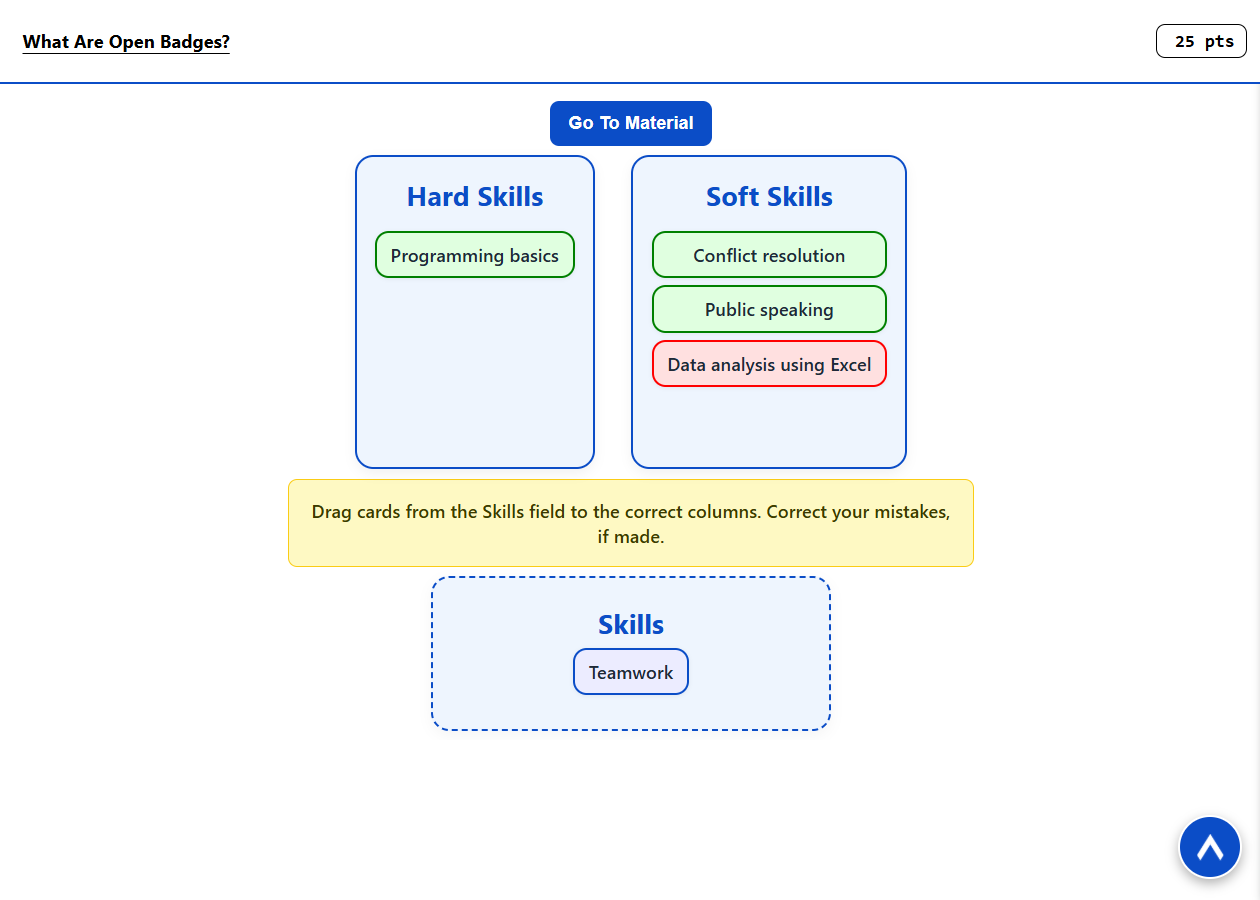
\includegraphics[width=0.8\textwidth]{Media/cards.png}
\caption{Card Sorting task in-progress}
\label{fig:cardTask}
{\raggedright \small{Source: created by the author, file src/tasks/cardTask.js}, 2025\par}
\end{figure}

Once all cards are placed correctly, the section is marked as complete, the score is persisted, the skills bank collapses and the task prompt is updated to state "Task completed!", to inform the user to continue with the next task. 
The parent TaskSection is notified via onUnlock(), allowing the next task to become accessible and the "Continue" button shows up for the user to conveniently progress.


\textbf{Task 2: Metadata Selection}

The second task introduces users to the structural components of an Open Badge by asking them to select only the necessary components of valid badge metadata. 
The goal is to reinforce understanding of which attributes are required for a badge to be considered valid and verifiable. 
Those elements are the issuer, badge earning criteria, issue date, encrypted recipient email, achievement description and badge class.

Here the task prompt is displayed at the top to be clearly visible and not interfere with the task display. 
It also appropriately updates upon completion.
This task uses a button grid for basic interactivity. 
Each enhance the simplicity of the task, each item appears as a button within a split “staircase” layout, which is displayed scaled based on the user's screen size whether on desktop or mobile.
The interaction is a set of ten shuffled elements, each mapped to either a valid metadata field or a plausible but incorrect distractor (e.g., “social media links”). 
When a user selects an option, the task validates whether it belongs to the Open Badge metadata schema. 
Correct answers trigger score gains and visually lock the button in place with a green highlight, and incorrect answers deduct points and display a feedback overlay with an explanation, using a mistakeKey.
A floating score bubble provides immediate feedback for each action as well.
An in-progress view of the task can be viewed in Figure \ref{fig:metadataTask}.

\begin{figure}[hbtp]
\centering
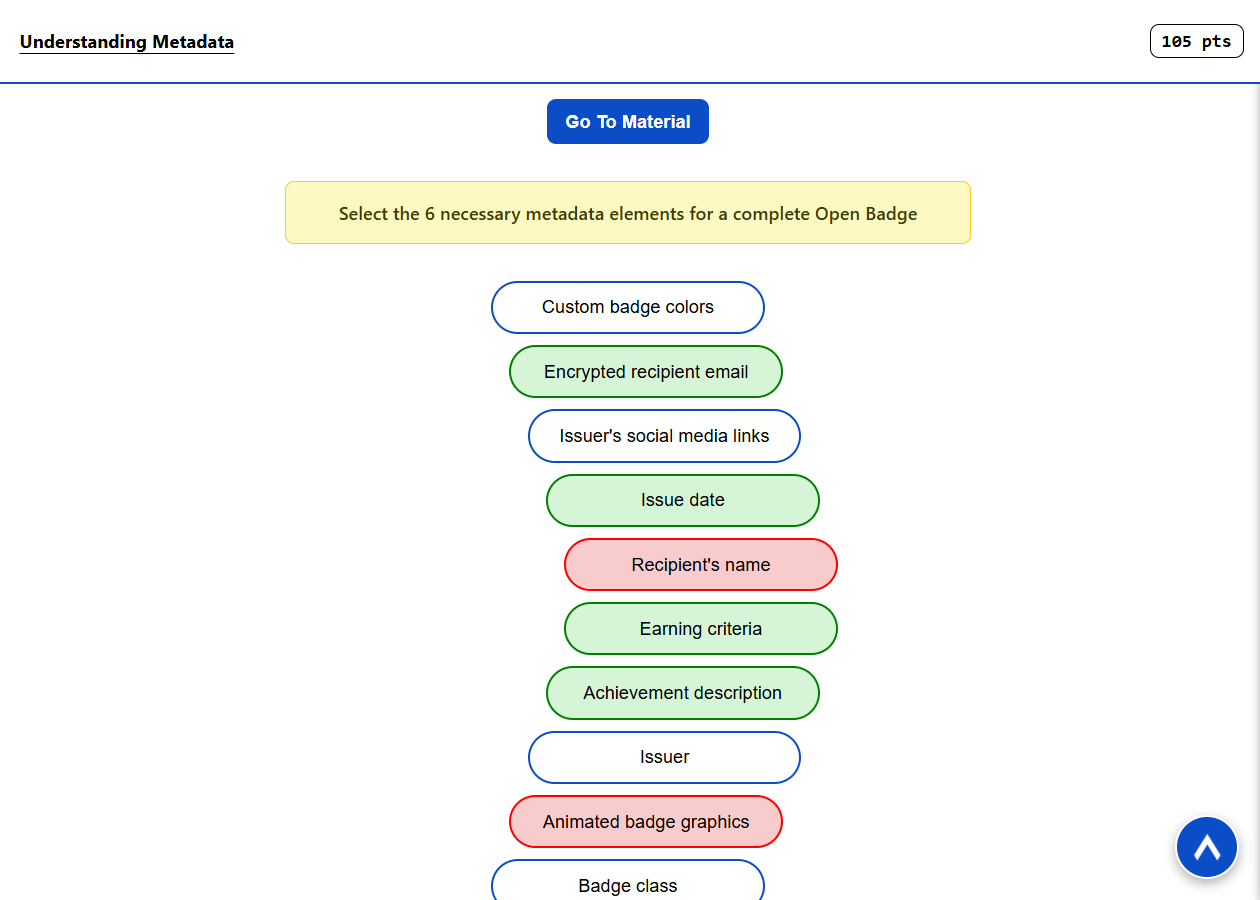
\includegraphics[width=0.8\textwidth]{Media/metadata.png}
\caption{Metadata Selection task in-progress}
\label{fig:metadataTask}
{\raggedright \small{Source: created by the author, file src/tasks/metadataTask.js}, 2025\par}
\end{figure}

The task uses internal state to track each selection (selected), and completion is detected once all correct elements have been chosen. 
As with other tasks, the system records progress using saveTaskCompletion(), locks the interface, and calls onUnlock() to reveal the next section.
Completion also triggers the "Continue" button to appear directly under the task, which would scroll down and realign the user at the next task.

 
\textbf{Task 3: Scenario-Based Selection}

The third task introduces contextual reasoning by asking users to select the most appropriate Open Badge for a given real-world scenario. 
It aims to deepen understanding of how badges represent specific competencies and apply to practical achievements. 
Each scenario presents a short narrative, followed by three visually distinct badge options, only one of which correctly reflects the competencies demonstrated in the story.
In retrospect, the received feedback pointed to this task being confusing to the user due to certain wording present within the scenarios, which caused mild frustration for a small number of users. 
After investigation, it was found that there were both a localization issue and a wording issue which was causing the frustration.
That leads to the conclusion that exact wording and maintenance of localisation are very important for an enjoyable experience.

The scenario logic is separated into a helper component, ScenarioSwiper.jsx, which manages animated transitions between scenarios using Framer Motion's <AnimatePresence> and <motion.div>. 
Only one scenario is rendered at a time, reducing distraction and allowing for focused attention. 
The swiper detects the current scenario via ID and animates horizontal transitions as users progress(select correct answers), simulating a card-swiping interface. 
Each badge option is rendered as a clickable button containing both text and an image of the corresponding badge. 
Like in previous tasks, selecting correct and incorrect answers will trigger the element to change colour and display a score delta, respectively. 
Each answer is locked after selection, so the user would not accidentally reduce their points, as the task does not progress until the correct answer, specifically, is selected.
Each scenario and possible answers are shuffled arrays to vary the orders across sessions. 
The in-progress view of the task can be seen in Figure \ref{fig:scenarioTask}. 
Once all three scenarios are answered correctly, the saveTaskCompletion() and onUnlock() functions are triggered, updating the task prompt and revealing the "Continue" button, as well as revealing the next section.

\begin{figure}[hbtp]
\centering
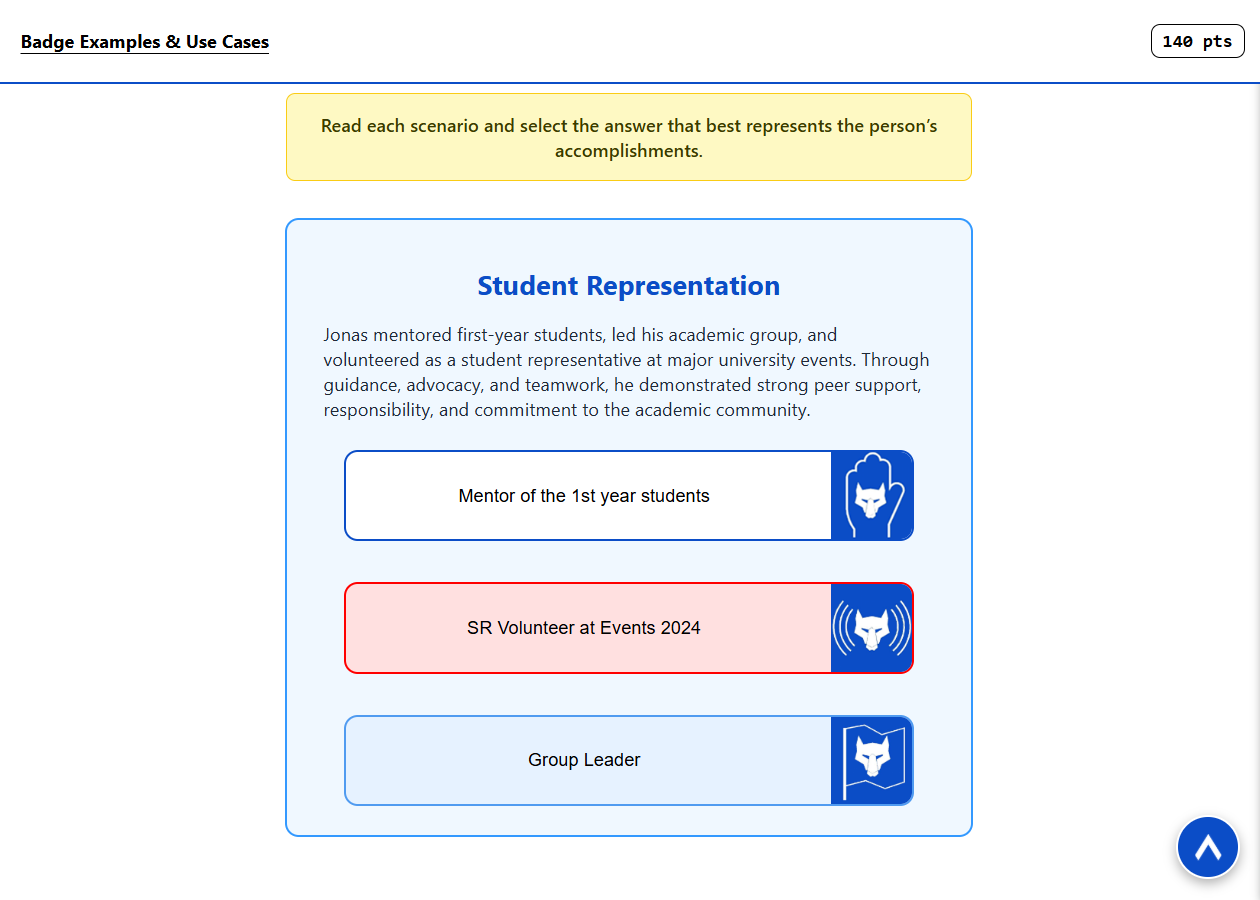
\includegraphics[width=0.8\textwidth]{Media/scenario.png}
\caption{Scenario-Based Selection task in-progress}
\label{fig:scenarioTask}
{\raggedright \small{Source: created by the author, file src/tasks/scenarioTask.js}, 2025\par}
\end{figure}


\textbf{Task 4: Badge Merging}

This task simulates the combination of smaller competence badges into a larger Meta badge. 
The user must drag smaller badge elements into a central slot, triggering a visual merge animation. 
The task builds on a key feature in badge ecosystems where multiple smaller achievements are combined into a badges of a new class, such as the "Meta" badge.
Notably, this task contains no possibility for incorrect answers, as such no mistake feedback is necessary.
This task is meant to function as a time for the user to relax, enjoy the animations and visual effects, and continue to the next and final task relatively quickly. 

In this task, users are presented with three smaller badges, a central merge zone (yellow circle, the \acrshort{cta} colour), as well as a task prompt instructing to drag the badges into the circle.
Using the @dnd-kit/core library again, learners are able to drag badges into the central drop area. 
The user interaction is handled through the DndContext, with each badge wrapped in a DraggableBadge component and the central area implemented as a DropZone. 
Internal state tracks which badges have already been placed and triggers a score reward via adjustScore() on each valid drop. 
Once all required badges are dropped, the task is marked complete, and a delayed animation video unlocks the next section after approximately seven seconds, allowing the user time to view the merge effect animation.
The animation that plays in question is a previous coursework project created with the intention of being used for this project specifically. 
It is a complex vector animation compiled as .MP4 file, that uses pre-loading as soon as the landing page is loaded for the user. 
The video is approximately 8 seconds long and is of approximately 700 KB in size, without loss in quality due to relatively simple vector graphics compression. 
A frame of the animation playing can be seen in Figure \ref{fig:mergeTask}, (b).

This task is supported by a helper component, MergeCenterDisplay, which handles dynamic text and visual content inside the merge zone based on drop progress. 
To represent the user's progress visually, the task uses a custom 
ProgressRing component. 
The ProgressRing component is called inside of MergeCenterDisplay. 
It is a React \acrshort{svg} that simply renders two circles, one of which is a static background circle, and the other one is a dynamic, green foreground circle, that is filled in based on user's progress, with a simple formula:
\progresscalc{current}{total}
Once dropped, each badge contributes to a looping animation that has the dropped badge icon orbiting within the inner area of the progress circle, on a select trajectory based on drop order, which can be seen in Figure \ref{fig:mergeTask} (a), simulating badge accumulation. 

\begin{figure}[H]
  \centering
  \begin{subfigure}[]{0.4\textwidth}
    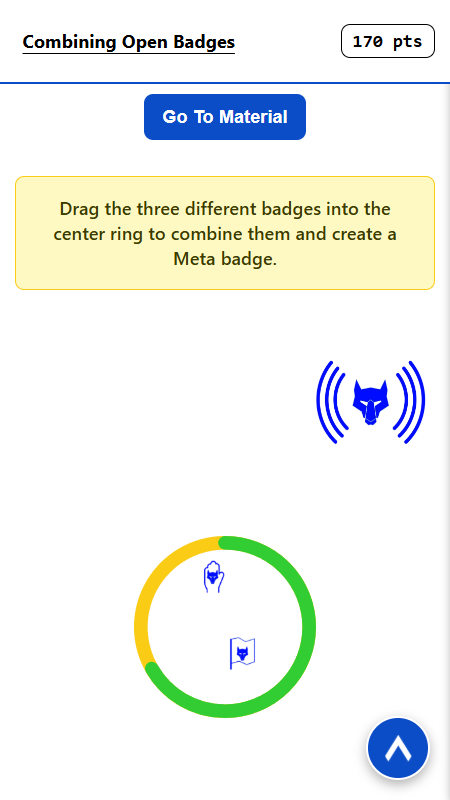
\includegraphics[width=\textwidth]{Media/merge1.png}
    \caption{Badge Merging in-progress}
  \end{subfigure}
  \hfill
  \begin{subfigure}[]{0.4\textwidth}
    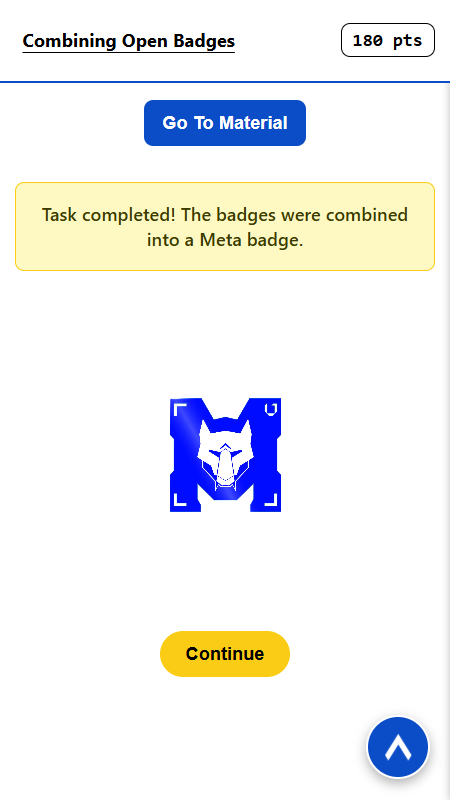
\includegraphics[width=\textwidth]{Media/merge2.png}
    \caption{Badge Merging post-completion animation playing}
  \end{subfigure}
  \caption{Badge Merging task, mobile view}
  \label{fig:mergeTask}
  {\raggedright \small{Source: created by the author, file src/tasks/mergeTask.js}, 2025\par}
\end{figure}


\textbf{Task 5: Card Classification}

The final task presents a sequence of statement cards related to the value and impact of Open Badges. 
Each card must be classified as either student-oriented or employer-oriented, reinforcing the dual value that Open Badges hold for both audiences. 
This final challenge ties together the learner’s understanding of badge value, communication and contextual application. 
The task is presented as a vertically stacked swiper or slider, where each card appears one at a time and offers two selectable categories ("Student", "Employer"). 
Correct classifications are locked in and trigger score feedback, and progress to the next card, while incorrect classifications trigger negative score feedback, providing visual guidance without penalising user flow. 
This leads to careful consideration without harsh interruption. 
The task in-progress can be viewed in Figure \ref{fig:swiperTask}.

\begin{figure}[hbtp]
\centering
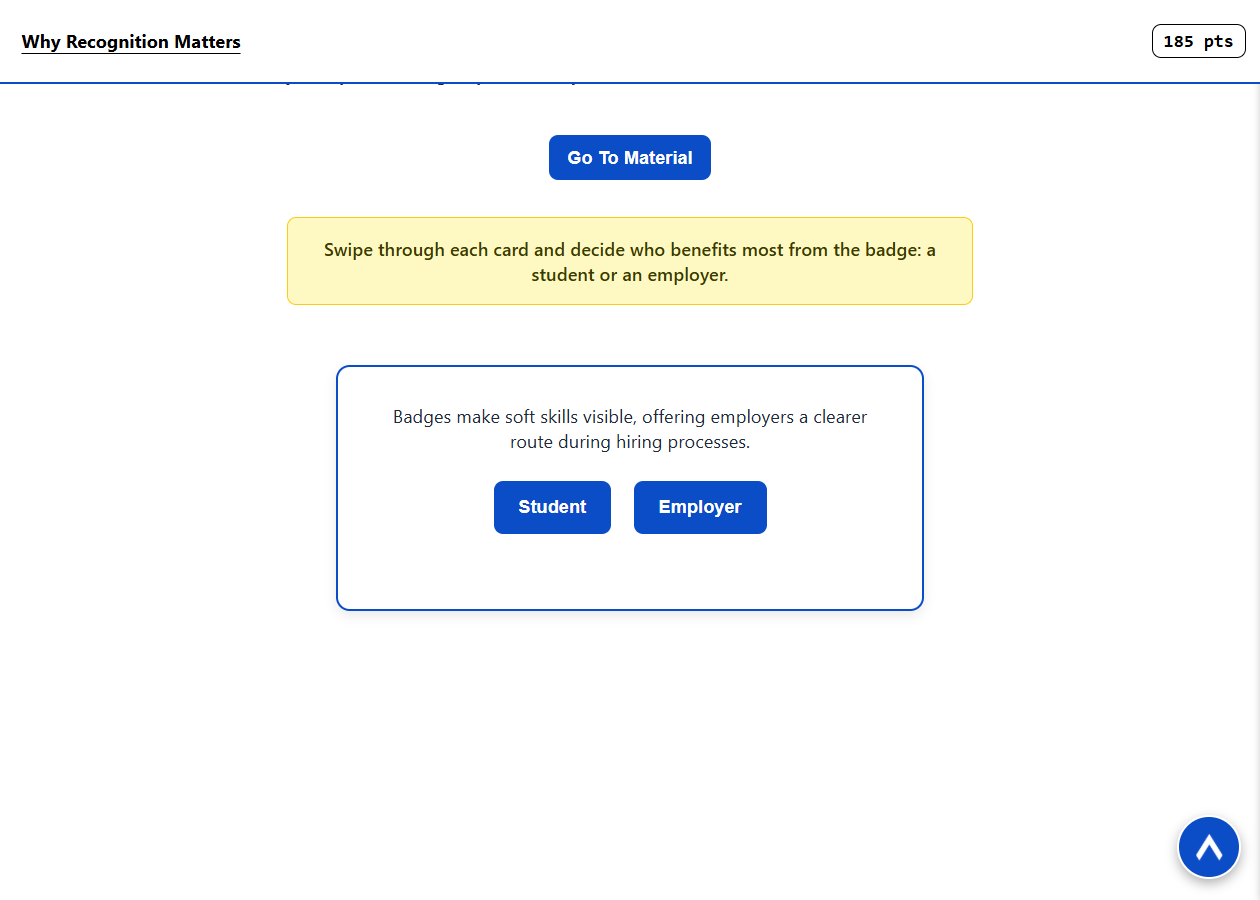
\includegraphics[width=0.8\textwidth]{Media/swiper.png}
\caption{Card Classification task}
\label{fig:swiperTask}
{\raggedright \small{Source: created by the author, file src/tasks/slidingTask.js}, 2025\par}
\end{figure}

Internally, each card's classification logic compares the selected category with a pre-defined key, which is either 0 or 1. 
The card slider is implemented using a dedicated helper component, slidingTaskHelper, which renders the current card, its classification options, and handles animations. 
It is very similar in structure to the scenarioSwiper but handles the elements differently. 
All correct classifications must be made to complete the task. 
Once completed, the task is locked, progress is stored, and the final "Finish" button appears to guide the user toward the badge issuance section. 
As with other tasks, all cards are shuffled on load using the shuffling function, to increase replayability. 

\subsubsection{End Section}

The final part of the website is only rendered upon completion of all tasks. 
This is tracked through local storage updates, checking for the task completion variable to include each section.
The section displays a basic form for the user's full name and email. 
The form utilises standard checks to ensure the user enters correct and viable information.
The submission button can only be triggered if the entered information is viable, which calls the backend with a request to issue an Open Badge for the user. 
The rest of this functionality is handled by the backend. 
The form gets replaced by the appropriate backend response based on the code returned, e.g. code 200 would lead to a success message or 500 would display an internal error message.
The end section additionally includes a "Play Again" button, which is a hold button, so the user wouldn't accidentally click it. 
After holding for a few seconds, the button scrolls the user to the top of the website while fading everything to white. 
Once the website is faded out, it wipes the user's accumulated total score and saved completed sections, then reloads the website so the tasks get reshuffled for a refreshed experience.

Together, these frontend technologies and design decisions form a responsive, gamified educational platform that adapts to user behaviour and supports pedagogical goals. By combining React’s modular strengths with carefully crafted gamified mechanics, the website delivers a rich and engaging learning experience across mobile and desktop devices.

\subsection{Backend Integration and Badge Issuance}

The backend of the gamified educational website was developed as an Express application using Node.js and deployed on Render.com platform as a lightweight, stateless \acrshort{api}. 
Its primary role is to securely manage and issue digital badges via the Open Badge Factory (from here - OBF) \acrshort{api}, while also supporting task verification and interaction logging. 
The backend architecture is purposefully minimal to preserve user privacy and reduce infrastructure complexity, with all sensitive operations encapsulated within server logic.

\subsubsection{Badge Issuance via Open Badge Factory API}

It was crucial to provide users with viable, verifiable and trusted Open Badges upon website completion. 
Due to technical limitations, it was not possible as of the time of writing this to integrate with the Vilnius Tech system on badgecraft.eu, so instead an alternative was chosen in Open Badge Factory. 
They utilise a Mozilla Open Badge standard for issuance, secured by OAuth-2, and allow for badge issuance automation via their \acrshort{api}, which is a perfect fit for the project. 
Upon form submission on the frontend, the frontend dispatches POST request containing the user’s email, name, final score, and language preference. 
This triggers a secure server-side sequence:

\begin{enumerate}
\item \textbf{Access Token Retrieval}: The backend authenticates itself by sending the preconfigured client\_id and client\_secret to OBF’s token endpoint at \textit{/client/oauth2/token} in an encoded format for security reasons. The full code of this retrieval can be seen in Figure \ref{fig:get_token}. 
If successful, a temporary OAuth-2 access token is returned. 
\begin{figure}[hbtp]
\centering
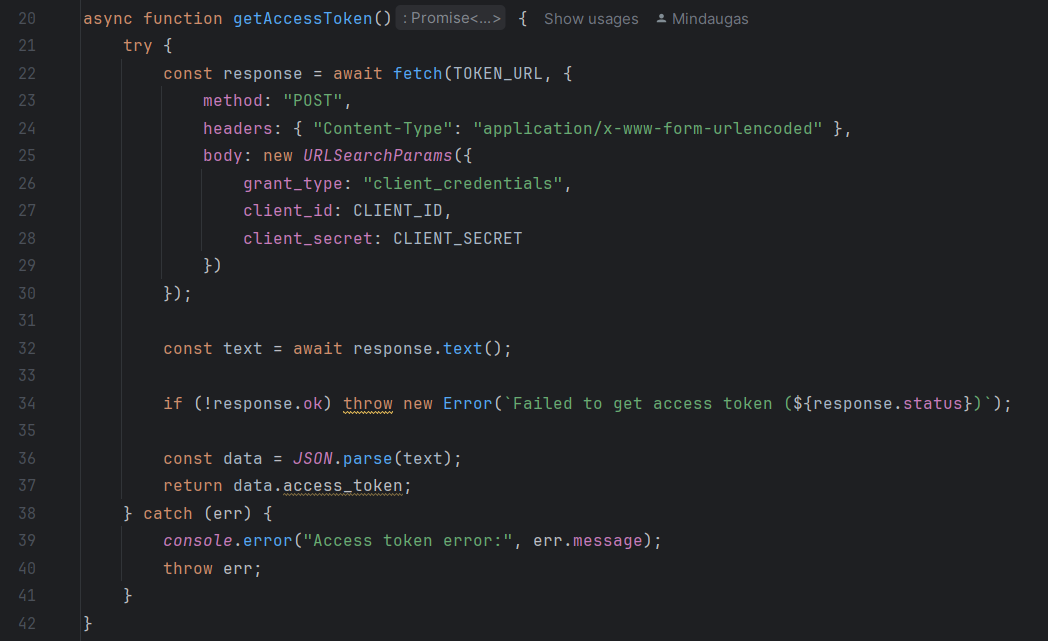
\includegraphics[width=0.8\textwidth]{Media/get_token.png}
\caption{Access Token retrieval backend function}
\label{fig:get_token}
{\raggedright \small{Source: created by the author, file backend/server.js, 2025}\par}
\end{figure}
\item \textbf{Existing Badge Check}: With the token, the server constructs and submits a GET request to OBF’s \textit{/client/client\_id/?email} endpoint. 
This returns a payload that includes issued badges and emails. 
The payload is then checked for a match within the payload and the user's submitted email. 
If a badge is already issued with the user's email, the error code of 409 is returned and a relevant message is delivered to the user on the frontend. 
Giving out multiple copies of the same badge, or even endlessly updating the badge would degrate the value of Open Badges. 
\item \textbf{Badge Issuance Request}: If the existing badge check gets passed, a new payload is created. 
It includes the access token, the user's name, email, submission date and individualised criteria addendum (updated with the user's final score) and a localised congratulations email(based on user's preference saved in local storage). 
Notably, additionally specified is the \textit{api\_consumer\_id = "standalone"}, which was not specified by the \acrshort{api} documentation as a necessary element to include, but in fact would consistently fail the issuance if excluded. 
This was discovered through extensive and thorough debugging. 
Its inclusion can be seen within the badge issuance payload in Figure \ref{fig:payload} and caused multiple setbacks during backend development.
The payload is then submitted as a POST request to \textit{/event/client\_id/badge\_id/issue}.
\item \textbf{Result Processing}: The backend verifies the response from OBF, logs the result internally, and returns a success or error message to the frontend. 
If the badge has already been issued for the user’s email, the backend returns a 409 status, preventing duplicates, a 200 status if the badge is successfully issued, or a 500 status for general errors.
\end{enumerate}
\begin{figure}[hbtp]
\centering
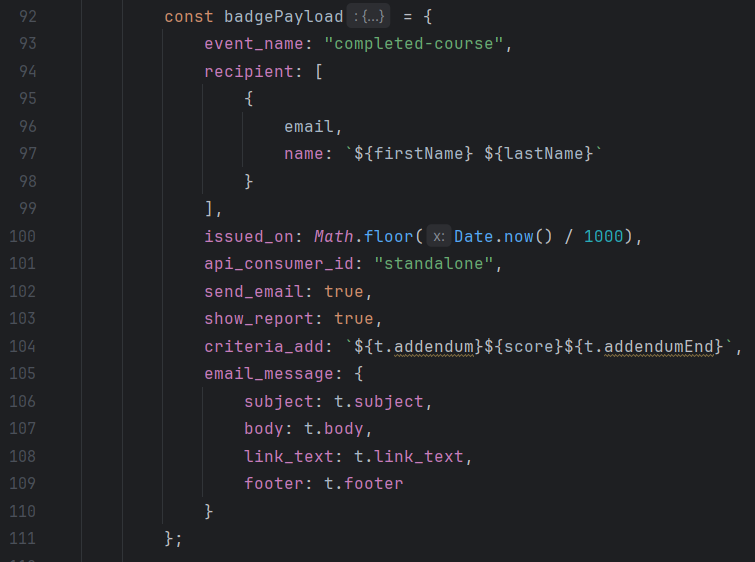
\includegraphics[width=0.8\textwidth]{Media/payload.png}
\caption{Badge issuance payload setup}
\label{fig:payload}
{\raggedright \small{Source: created by the author, file backend/server.js}, 2025\par}
\end{figure}
The client secrets are handled exclusively within the backend environment. 
This architecture ensures that no sensitive client secrets are ever exposed to the browser, because if it were handled via frontend, which is also possible, React framework would expose all environment variables. 
All credentialed communication with the Open Badge Factory occurs strictly server-side, maintaining full compliance with security best practices. 
The badge response is formatted in \acrshort{json} and parsed before returning a confirmation message to the user-facing application.

\subsubsection{Session Logging and Progress Tracking}

To support analytics and debugging without requiring user authentication, the website implements session-based logging. 
On first load, a unique session identifier is generated on the frontend and stored in local storage. 
This session ID is attached as the header to all of the log messages and progress data that will eventually get sent to the backend.
As previously discussed, each significant event, such as score adjustments, task completions, or badges, is logged through a backend endpoint at \textit{/api/log} that receives structured \acrshort{json} payloads. These logs are:

\begin{itemize}
\item Persisted as individual session files in the directory.
\item Indexed by session ID for traceability and analysis.
\item Accessible via a read-only interface for development and analysis review.
\end{itemize}

This setup allows the system to track meaningful interactions while avoiding the storage of personally identifiable information (PII), maintaining both privacy and transparency. 
Notably, during testing, an issue occurred where the backend server would come down for maintenance, and the storage solution did not prove to be persistent. 
Luckily, the terminal was persistently tracking submission, and all relevant data were successfully recovered. 
For a future reimplementation with Vilnius Tech, this would have to be reviewed based on the technology available. 
A sample log includes fields such as:

\begin{itemize}
\item Unique session identifier.
\item Total user score at submission.
\item UTC timestamp for badge issuance event (if applicable).
\item A counter of correct and incorrect answers.
\item Array of event objects, each containing event type, timestamp, and metadata for score changes.
\end{itemize}

\subsubsection{API Design and Structure}

The backend exposes a set of endpoints summarised as follows:
\begin{itemize}
\item Badge issuance via OBF’s \acrshort{api} with the endpoint \textit{/api/issue-obf-badge}.
\item Accepts structured interaction logs from the frontend and saves them to the backend upon completion at \textit{/api/log}.
\item Retrieves a single session’s full event log for testing and analysis purposes at \textit{/api/logs/:sessionId}.
\item Lists summaries of all stored sessions for basic analytics at \textit{/api/sessions}.
\end{itemize}
No personal user data is collected unless voluntarily provided for badge issuance (e.g., email), which is stored transiently and passed directly to the OBF API. 

\subsection{Technical Limitations}

While the system successfully delivers an engaging and functional gamified learning experience, a number of technical limitations were encountered during implementation that shaped design decisions and constrained the project.

First, the backend operates without persistent user accounts or authentication mechanisms and the free or cheap(there was a necessary switch during development) hosting service utilised for the project has caused both consistency and persistence issues. 
Therefore, all information is saved locally until it is delivered to the server, where currently some of the data has to be checked and stored elsewhere manually in case of the hosting service's forced redeployment of the backend. 
While the backend is lightweight, private for the end-user, fast and functional, it introduces a certain degree of fragility which should be considered upon final integration into a system. 
Additionally, currently, badge reissuance is not possible without administrative intervention or additional verification.

Second, although initial plans considered integrating with Vilnius Tech’s internal badge infrastructure, the decision was made to issue Open Badges via the external Open Badge Factory (OBF) API. 
This change was due to technical and institutional constraints, including a lack of public badge-issuing endpoints on badgecraft.eu (the system provider for Vilnius Tech) and limited documentation within the university system. OBF provided a reliable and standards-compliant alternative, albeit with its own integration challenges. 
The \acrshort{api} access on OBF is also exclusive to a paid service. 
For development purposes, an extensive trial was available to create a proof-of-concept. 
In the future, however, badge delivery is expected to be unavailable, unless the change to badgecraft.eu is completed.

Third, the badge claiming process relies on user-provided data, submitted through a frontend form. 
Although basic validation is applied, there is no real-time email verification or confirmation step, which opens the possibility of incorrect or unverified badge claims. 
Additionally, it is difficult to verify the person who claimed the actual badge without more tools. Future implementations could mitigate this by integrating optional email confirmation using institutional SSO authentication systems, if available.

On the frontend, ensuring responsive and interactive behaviour across various screen sizes, especially for mobile-first design, required extensive custom logic. 
Scroll-triggered visual effects, such as the animated \acrshort{svg} zigzag path and section snapping behaviours, were particularly complex to tune across mobile browsers with varying scroll engines and event handling. 
Inconsistent behaviour was occasionally observed, particularly on niche phone models where an extremely narrow screen would have the text elements bleed into each other, causing the relevant and relative \acrshort{svg} elements to draw over the text.

Additionally, while interaction logs are captured via a local event logger and submitted alongside the badge claim, the absence of integrated analytics tools limits fine-grained insights into user behaviour, task completion time, and drop-off rates. 
This makes it more difficult to empirically assess which sections present challenges to learners or which features are most engaging. 
Notably, drop-off points were also not investigated within the testing section as well as they were considered out of scope, due to the small sample size.

With all of the technical limitations considered, the final product was still well received and achieved the necessitated goals to an extent that will be further discussed within the testing section.

\newpage